\documentclass[letterpaper,11pt,oneside,titlepage]{report}
\usepackage{mathtools,amsfonts,amssymb,amsthm}
\usepackage[utf8]{inputenc}
\usepackage{graphicx,float,epstopdf,xcolor}
\usepackage{lastpage}
\usepackage[font=small]{subcaption}
\usepackage{caption}

\floatstyle{plaintop}
\restylefloat{table}
%A drawback of this is that you can't have more than one caption per table, i.e. you can't have two different tabulars with two captions side-by-side (question 22751 tex.stackexchange.com)


\usepackage{tabularx}
\usepackage[left=2cm,top=3cm,right=2cm,bottom=3cm]{geometry} 

\usepackage{sansmathfonts}
\usepackage{helvet}
\renewcommand{\familydefault}{\sfdefault}

\usepackage{titlesec}
\titleformat{\chapter}[display]
{\normalfont\bfseries\centering}{\chaptertitlename\ \thechapter}{12pt}{\MakeUppercase}

%-----------------------------------------------------

\newcommand{\reportnumber}{TR-02-2024}
\newcommand{\reporttitle}{FLEXODEAL-LITE V0.1: SOLVER PERFORMANCE FOR DYNAMIC PASSIVE NEO-HOOKEAN DEFORMATION}


%-----------------------------------------------------


%\usepackage{lipsum}

\usepackage{fancyhdr}
\fancypagestyle{trheadings}{
  \fancyhf{}
  \renewcommand{\headrulewidth}{0pt}
  \fancyhead[L]{NEUROMUSCULAR MECHANICS LABORATORY}
  \fancyhead[R]{Page \thepage/\pageref*{LastPage}}
  \fancyfoot[C]
  {
    \begin{tabularx}{\textwidth}{|>{\centering\arraybackslash}X|c|}\hline 
    \textbf{TECHNICAL REPORT \reportnumber} & Total Pages\\[0.5em]
    \reporttitle & \pageref*{LastPage} \\\hline
    \end{tabularx}
  }
}

\makeatletter
\renewcommand\chapter{\if@openright\cleardoublepage\else\clearpage\fi
                    \thispagestyle{fancy}% original style: plain
                    \global\@topnum\z@
                    \@afterindentfalse
                    \secdef\@chapter\@schapter}
\makeatother

\def\labelitemi{--}


\usepackage{hyperref}
\usepackage{stmaryrd}
\SetSymbolFont{stmry}{bold}{U}{stmry}{m}{n} % 

%-----------------------------------------------
% Eliminate ugly boxes around references.
\hypersetup{
    colorlinks,
    linkcolor={red!50!black},
    citecolor={blue!50!black},
    urlcolor={blue!80!black}
}
%------------------------------------------------

%------------------------------------------------
\newtheorem{theorem}{Theorem}[chapter]
\newtheorem{lemma}[theorem]{Lemma}
\newtheorem{corollary}[theorem]{Corollary}
\newtheorem{remark}[theorem]{Remark}

\renewcommand{\theremark}{\thechapter.\arabic{remark}}
\renewcommand{\thetheorem}{\thechapter.\arabic{theorem}}
\renewcommand{\thelemma}{\thechapter.\arabic{lemma}}
\renewcommand{\thecorollary}{\thechapter.\arabic{corollary}}
%------------------------------------------------


%%%%%%%%%%%%%%%%%%%%%%%%%%%%%%%%%%%%%%%%%%%%%%%%%%%
%
%	WATERMARK
%
%%%%%%%%%%%%%%%%%%%%%%%%%%%%%%%%%%%%%%%%%%%%%%%%%%%
%\usepackage{draftwatermark}
%\SetWatermarkText{DRAFT}
%\SetWatermarkScale{1.3}
%\SetWatermarkLightness{0.94}
%\usepackage{lmodern} % To remove the warning from unavailable font shape

%%%%%%%%%%%%%%%%%%%%%%%%%%%%%%%%%%%%%%%%%%%%%%%%%%%
%
%  DEFINITIONS 
%
%%%%%%%%%%%%%%%%%%%%%%%%%%%%%%%%%%%%%%%%%%%%%%%%%%%

%\def\*#1{{\mathbf{#1}}} % bold letters!


%%%%%%%%%%%%%%%%%%%%%%%%%%%%%%%%%%%%%%%%%%%%%%%%%%%
%
% END OF DEFINITIONS
%
%%%%%%%%%%%%%%%%%%%%%%%%%%%%%%%%%%%%%%%%%%%%%%%%%%%



\begin{document}
\thispagestyle{empty}
\setlength{\footskip}{36pt}


\begin{titlepage}

\center % Center everything on the page
 
%----------------------------------------------------------------------------------------
%	HEADING SECTION
%----------------------------------------------------------------------------------------
\vspace*{-6.5em}

\noindent\begin{minipage}[t]{0.69\textwidth}
\textbf{SIMON FRASER UNIVERSITY} \\
\textbf{DEPARTMENT OF BIOMEDICAL PHYSIOLOGY AND KINESIOLOGY} 
\end{minipage} \hfill
\begin{minipage}[r]{0.29\textwidth}
\begin{flushright}
\vspace*{-0.1cm}

\includegraphics[width=0.5\textwidth]{logos/sfu-logo.eps}
\end{flushright}
\end{minipage}

%----------------------------------------------------------------------------------------
%	TITLE SECTION
%----------------------------------------------------------------------------------------

\vfill

\begin{minipage}[c]{0.8\textwidth}
\centering
\large \textbf{NEUROMUSCULAR MECHANICS LABORATORY} \\[1em]
\large \textbf{TECHNICAL REPORT \reportnumber}\\[2em]

\includegraphics[width=0.3\textwidth]{logos/nml-logo.png}
\end{minipage}

\vspace{8em}

\begin{minipage}[c]{0.8\textwidth}
\centering
\large \textbf{\reporttitle}
\end{minipage}

\vfill
 
%----------------------------------------------------------------------------------------
%	AUTHOR SECTION
%----------------------------------------------------------------------------------------

\begin{tabularx}{\textwidth}{|X|X|X|}\hline
\textbf{AUTHOR(S):} & \textbf{REVISED BY}: & \textbf{APPROVED BY:} \\[0.5em]
Javier Almonacid &  &  \\[0.5em]\hline
\textbf{LAST UPDATED:} & \textbf{LAST REVISION:} & \textbf{DATE APPROVED:} \\[0.5em]
\today &  &  \\[0.5em]\hline
\end{tabularx}\\[2em]

\begin{tabularx}{\textwidth}{|>{\centering\arraybackslash}X|c|}\hline 
  \textbf{TECHNICAL REPORT \reportnumber} & Total Pages\\[0.5em]
  \reporttitle & \pageref*{LastPage} \\\hline
\end{tabularx}

\vspace{-4.28em}

\end{titlepage}


\pagestyle{trheadings}
\titleformat{\chapter}
{\normalfont\Large\bfseries}{\thechapter. }{0pt}{\Large}
\setlength{\headheight}{14pt}
\titlespacing*{\chapter}{0pt}{-24pt}{12pt}
\setlength{\parskip}{1em}
\titleformat*{\section}{\bfseries}
\titleformat*{\subsection}{\bfseries}
\setcounter{page}{2}


%--------------------------------------------

\chapter{Executive Summary}
\setlength{\parskip}{0.5em}

TBD


%--------------------------------------------
\cleardoublepage
\setlength{\parskip}{0pt}
{\hypersetup{linkcolor={black!50!black}}


%\addcontentsline{toc}{section}{Resumen}
\tableofcontents 

%\cleardoublepage
%\addcontentsline{toc}{chapter}{List of Figures}
%\listoffigures 

%\cleardoublepage
%\addcontentsline{toc}{chapter}{List of Tables} 
%\listoftables

%------------------------------------

\chapter{Overall description of v0.1}

The code begins from a dynamic extension of step-44 available at
\begin{center}
  \url{https://github.com/javieralmonacid/dynamic-step-44}. 
\end{center}

First, the geometry is changed from the cube considered in step-44 to a more general hyper-rectangle (in deal.II's terminology) of length, width, and height provided in the parameters file. Then we implement a simple boundary condition for pushing/pulling which we describe below. Finally, in addition to the CG and Direct (UMFPACK) solvers implemented by default in step-44, we implement the GMRES solver.

\section{Linear pull/push profile}

First, we assume the standard colouring of faces for the hyper-rectangle, i.e. -x face = boundary ID 0, +x face = 1, -y face = 2, +y face = 3, -z face = 4, +z face = 5. Then, on the +x face of the block, given a start time $t_{start}$, an end time $t_{end}$, a maximum strain $\lambda_0$, a pulling/pushing strain rate $\epsilon_0$, and a muscle length $L_0$, we prescribe the following length profile:
\begin{equation}
  L(t) = \left\{ \begin{aligned}
    &L_0 \quad &&t_{start} \leq t \leq t_0, \\
    &\mathrm{sign}(\lambda_0) \epsilon_0 (t-t_*) + L_* \quad &&t_0 < t < t_1, \\
    &L_1 \quad &&t_1 \leq t \leq t_{end}.
  \end{aligned} \right.
\end{equation}
Here,
\[
  t_* = \dfrac{t_{start}+t_{end}}{2}, \quad L_* = \dfrac{L_0+L_1}{2}, \quad L_1 = \lambda_0 (1+L_0).
\]
Moreover, if $L_1 > L_0$ (i.e. when pulling),
\[
  t_0 = \dfrac{L_0-L_*}{\epsilon_0} + t_*, \quad t_1 = \dfrac{L_1-L_*}{\epsilon_0} + t_*.
\]
In turn, if $L_0 > L_1$ (i.e. when pushing),
\[
  t_0 = \dfrac{L_1-L_*}{\epsilon_0} + t_*, \quad t_1 = \dfrac{L_0-L_*}{\epsilon_0} + t_*.
\]
The idea is that the line defining the length for times $t_0 < t < t_1$ never surpasses $L_0$ or $L_1$. This means that $t_0 \geq t_{start}$ and $t_1 \leq t_{end}$, which can be enforced by asking that
\[
  \epsilon_0 \geq \left| \dfrac{\lambda_0 L_0}{t_{end}-t_{start}} \right|.
\]
The displacement boundary condition is then simply $\mathbf{u}_D = (u_D,0,0)$, with $u_D(t) = L(t) - L_0$. The remaining boundary conditions are:
\begin{itemize}
  \item -x face: clamped in all three directions.
  \item -y, +y, -z, +z faces: traction free.
\end{itemize}

\chapter{Numerical results (passive experiments)}

We consider the following parameters :
\begin{itemize}
  \item Geometry $[0,3] \times [0,1] \times [0,1]$ with a scaling parameter of 1e-03\footnote{The scaling parameter only affects the geometry of the block and not its material properties.}
  \item \textbf{set Type of simulation = dynamic}
  \item set Polynomial degree = 2
  \item set Quadrature order  = 5
  \item Global refinement level = 3
  \item set Pressure ratio p/p0 = 0 
  \item set Max iteration multiplier = 2
  \item set Residual                 = 1e-6 (linear solver residual)
  \item \textbf{set Use static condensation = false}
  \item set Preconditioner type  = ssor
  \item set Preconditioner relaxation  = 0.65
  \item \textbf{set Solver type              = Direct}
  \item set Poisson's ratio = 0.4999
  \item set Shear modulus   = 80.194e6
  \item set Max iterations Newton-Raphson = 20
  \item set Tolerance displacement        = 1.0e-6
  \item set Tolerance force               = 1.0e-9
  \item set End time       = 0.525
  \item set Time step size = 0.025
  \item set Pulling face ID  = 1
  \item set Pull time start  = 0.0
  \item set Pull time end    = 0.5
  \item set Pull strain      = -0.15
  \item set Pull strain rate = 0.00090
\end{itemize}

The solver computes results in 272.8 seconds. We portray them next.

\begin{figure}
  \centering
  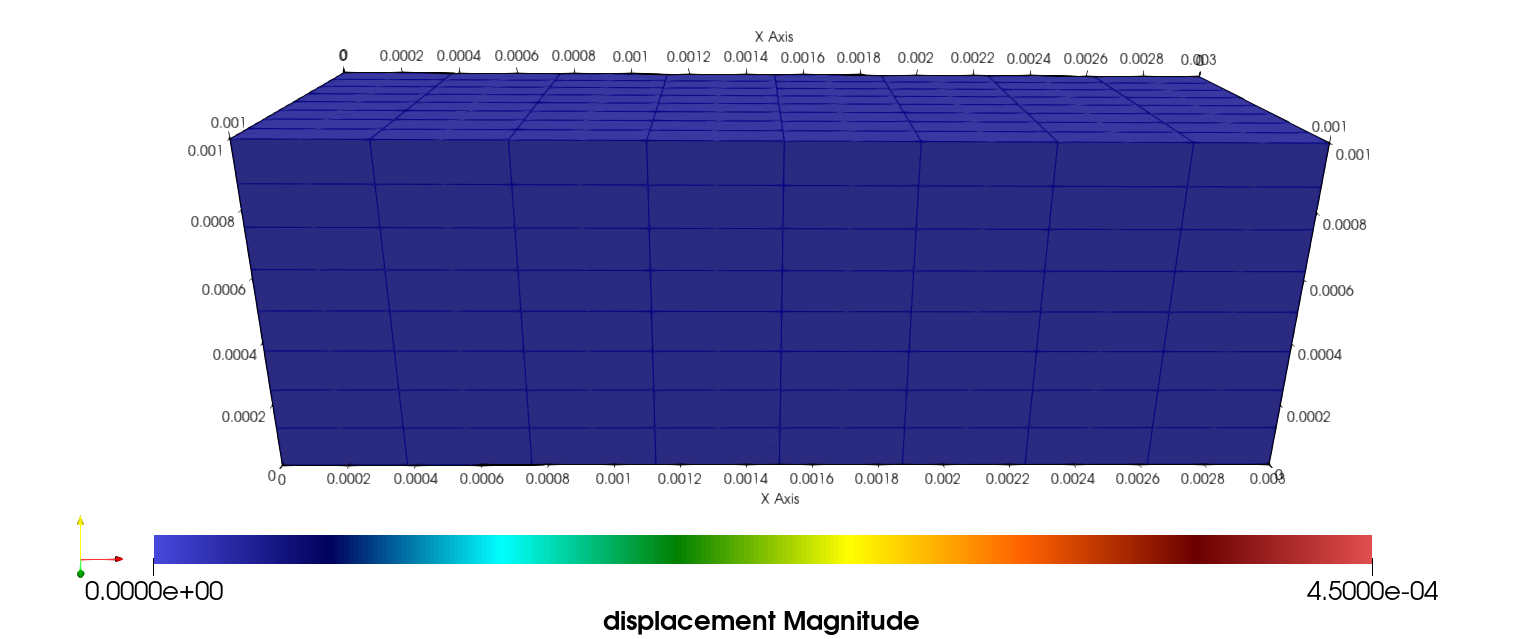
\includegraphics[height=0.18\textheight]{figs/00-u.png}
  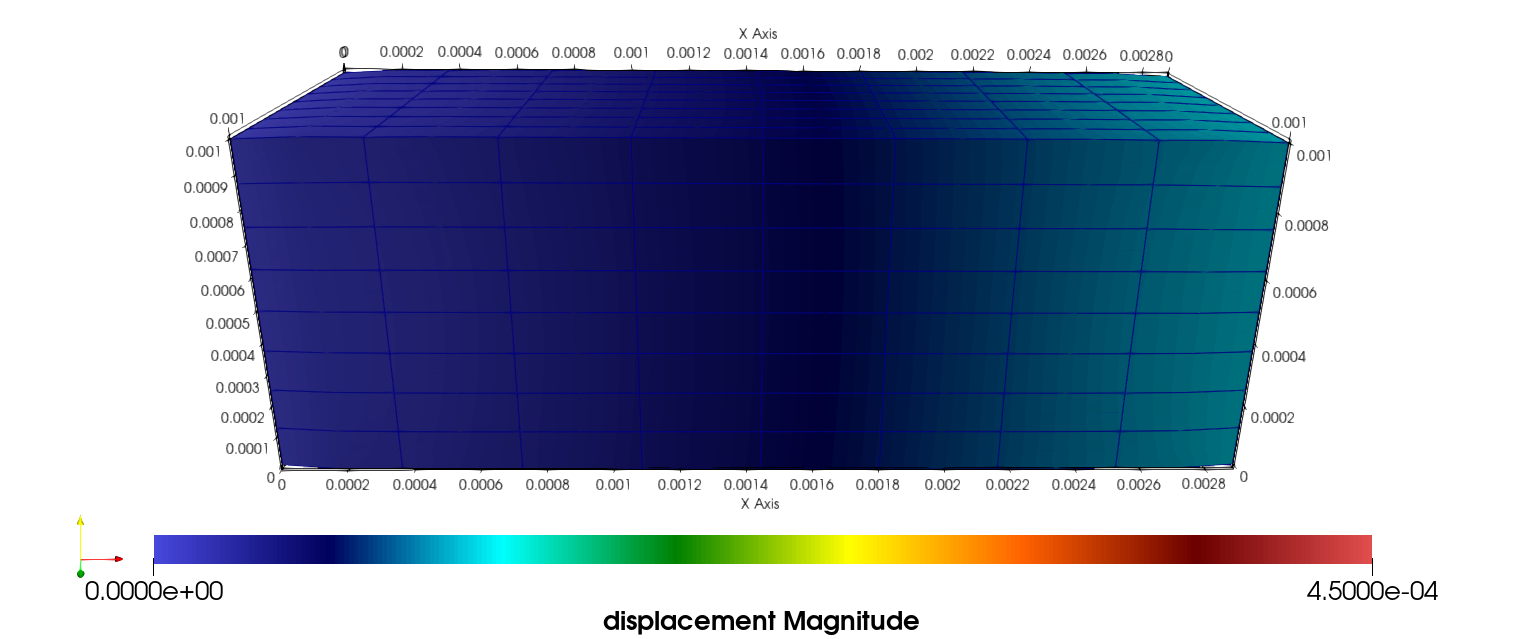
\includegraphics[height=0.18\textheight]{figs/05-u.png}
  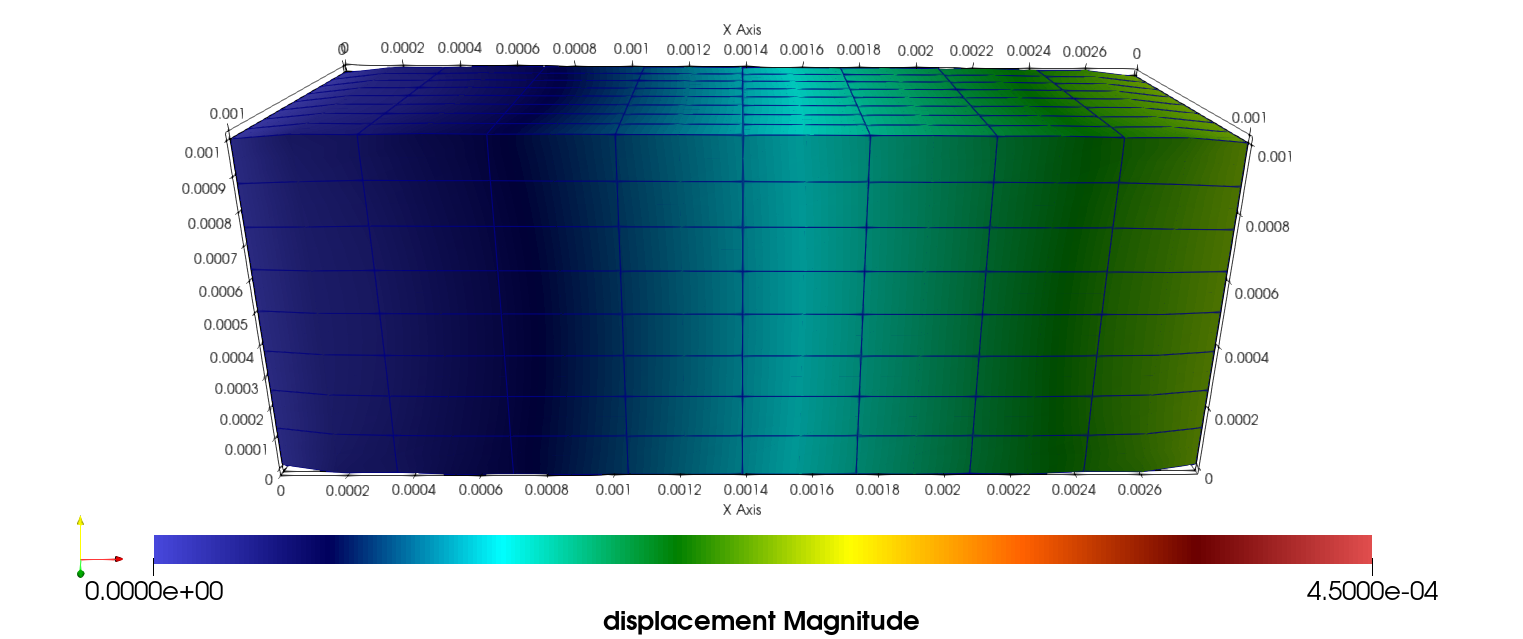
\includegraphics[height=0.18\textheight]{figs/10-u.png}
  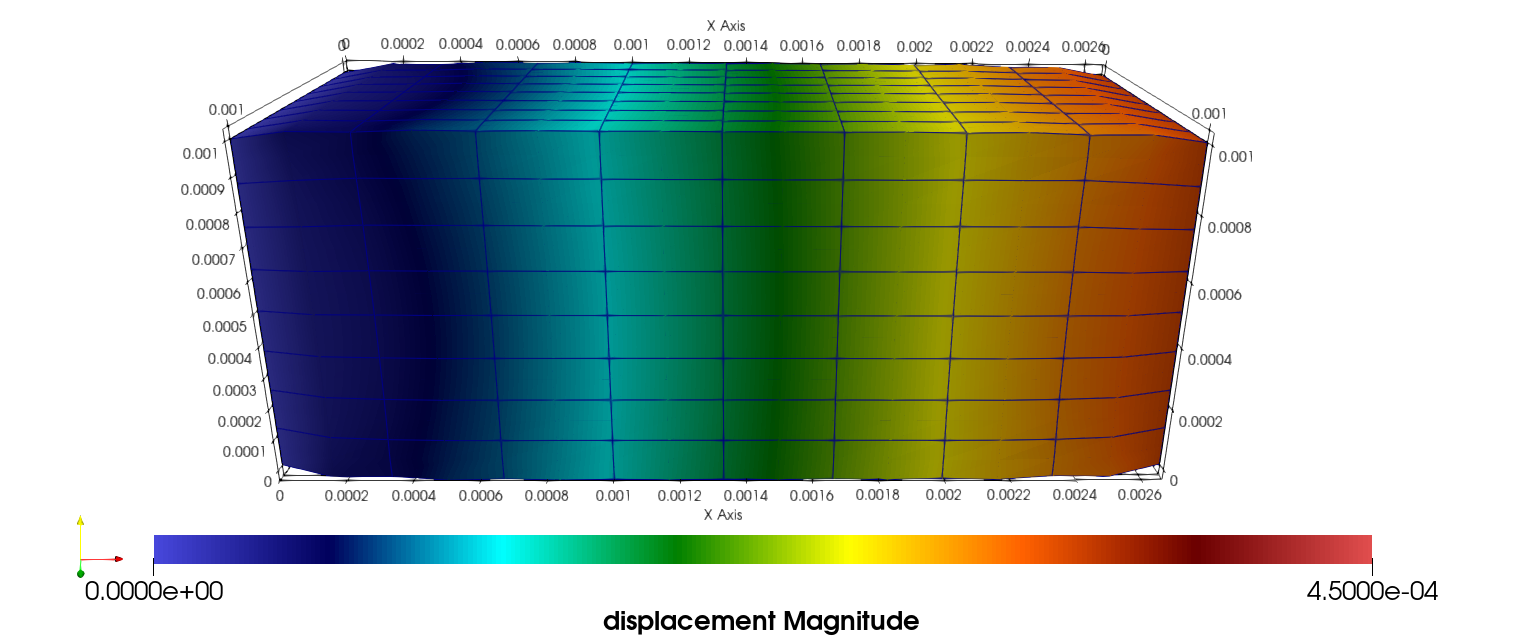
\includegraphics[height=0.18\textheight]{figs/15-u.png}
  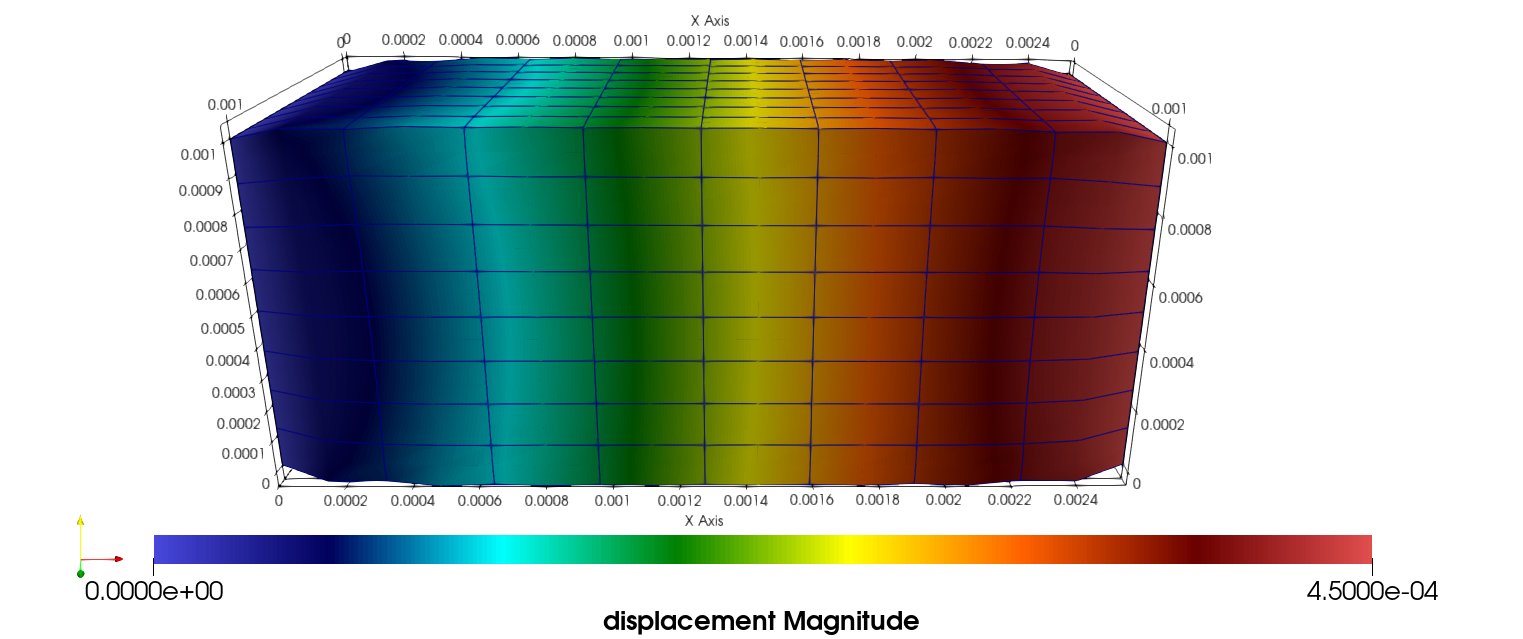
\includegraphics[height=0.18\textheight]{figs/20-u.png}
  \caption{Screenshots of displacement at timesteps 0 of 20, 5 of 20, 10 of 20, 15 of 20, and 20 of 20.}
\end{figure}

\begin{figure}
  \centering
  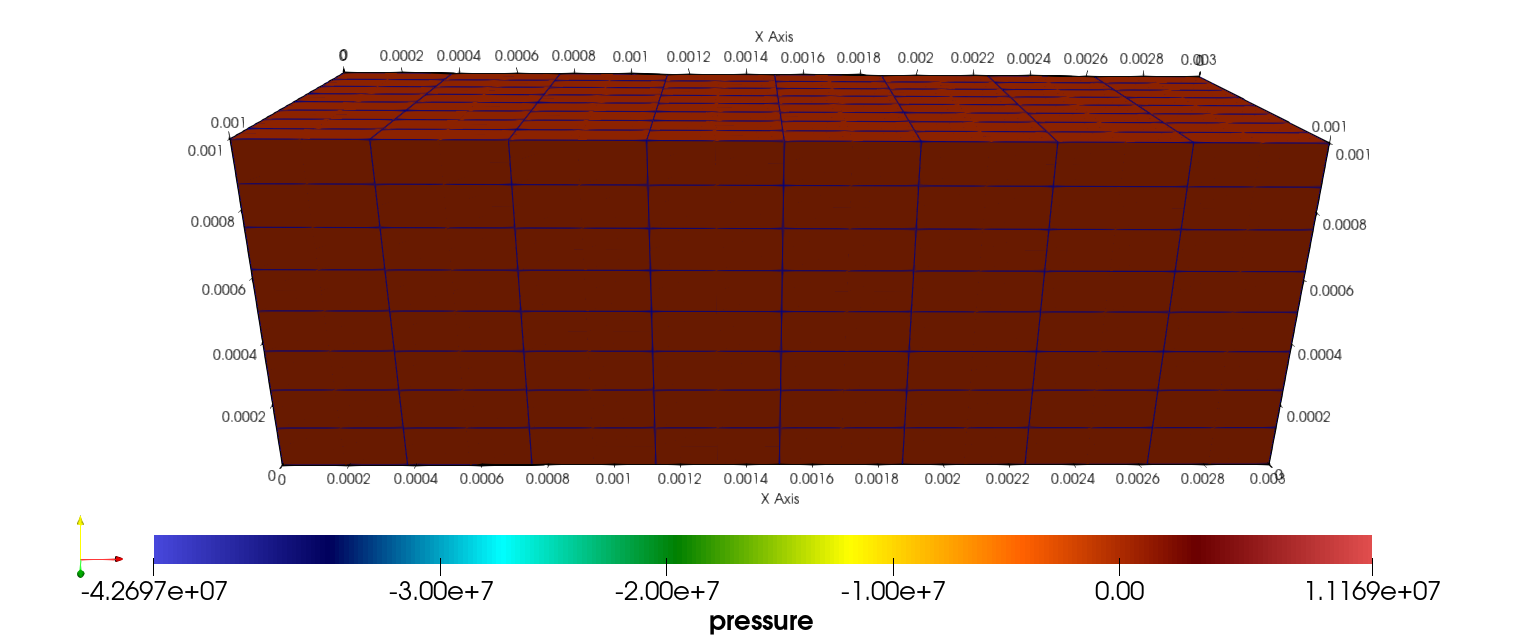
\includegraphics[height=0.18\textheight]{figs/00-p.png}
  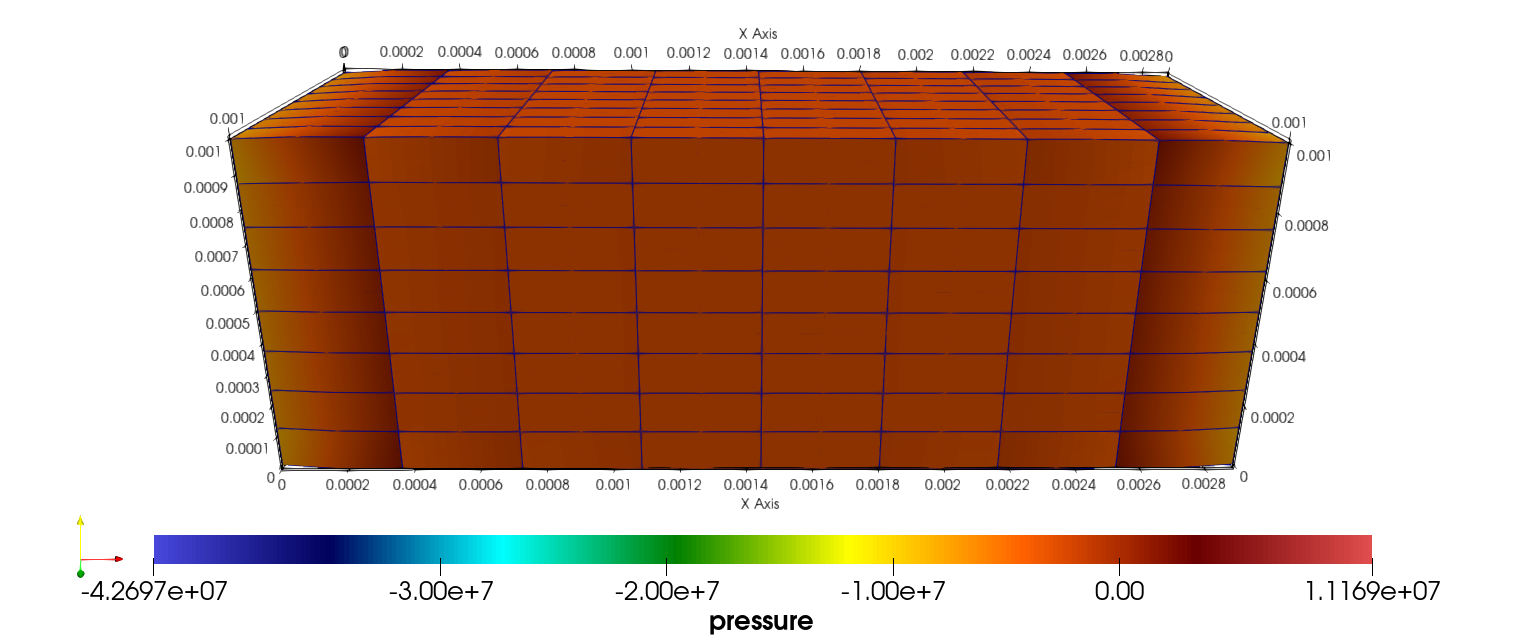
\includegraphics[height=0.18\textheight]{figs/05-p.png}
  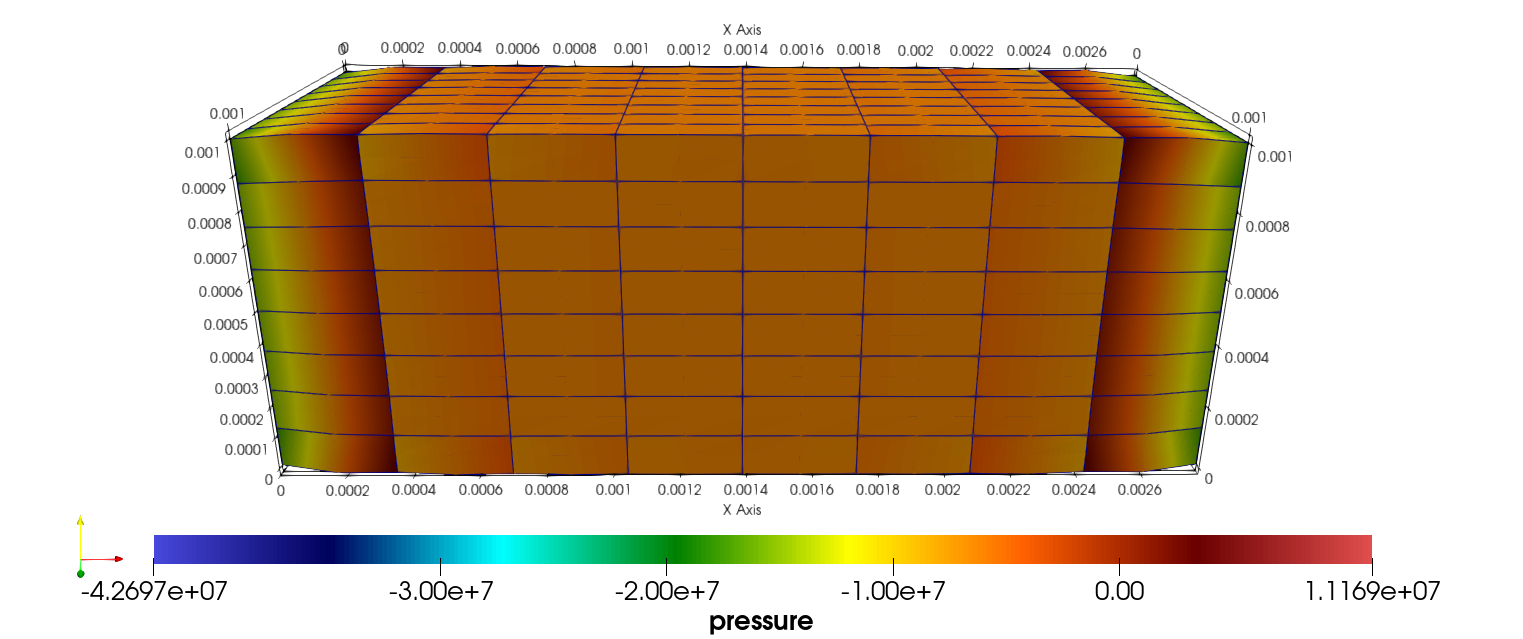
\includegraphics[height=0.18\textheight]{figs/10-p.png}
  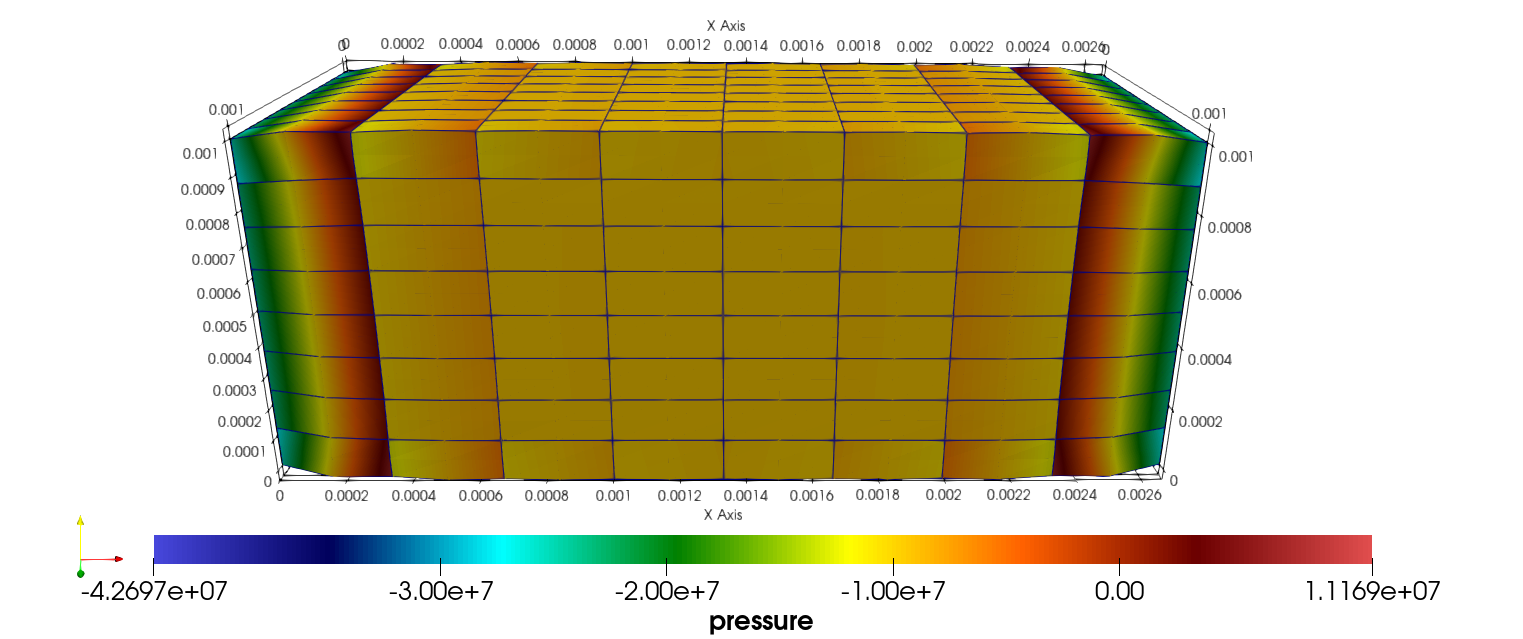
\includegraphics[height=0.18\textheight]{figs/15-p.png}
  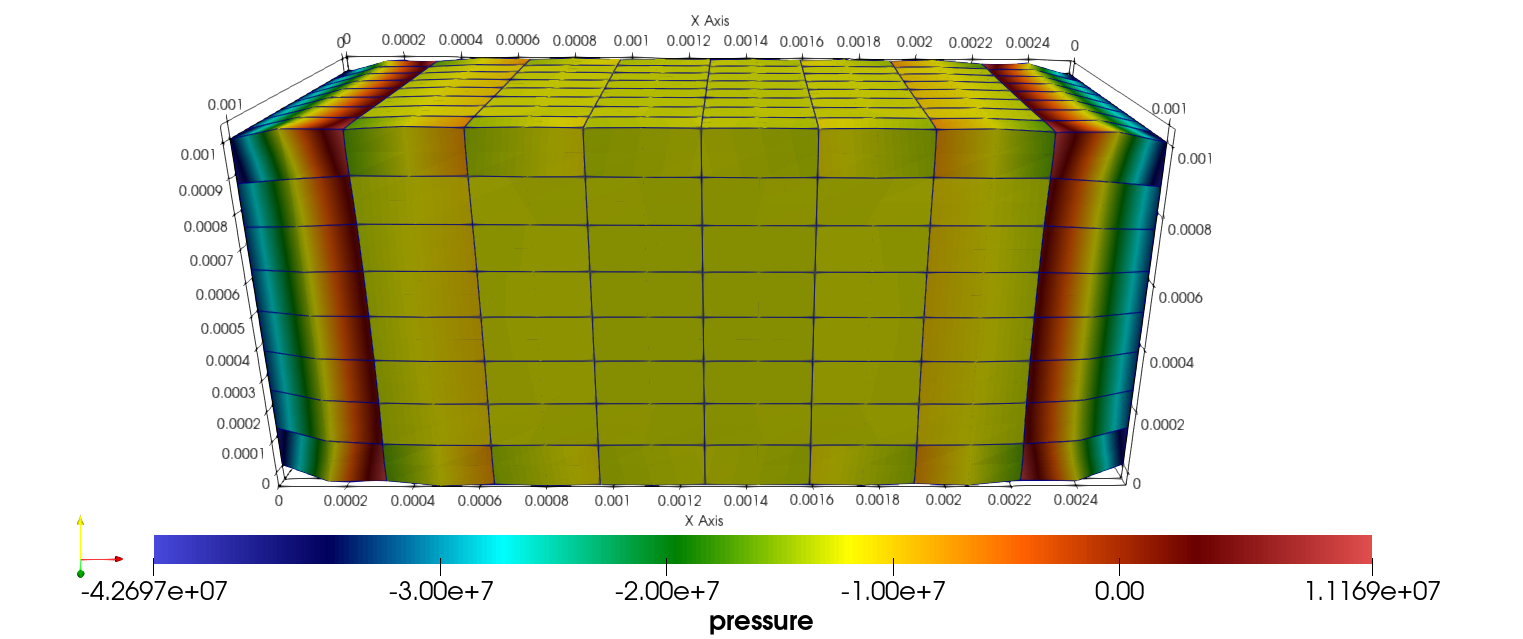
\includegraphics[height=0.18\textheight]{figs/20-p.png}
  \caption{Screenshots of pressure at timesteps 0 of 20, 5 of 20, 10 of 20, 15 of 20, and 20 of 20.}
\end{figure}

\begin{figure}
  \centering
  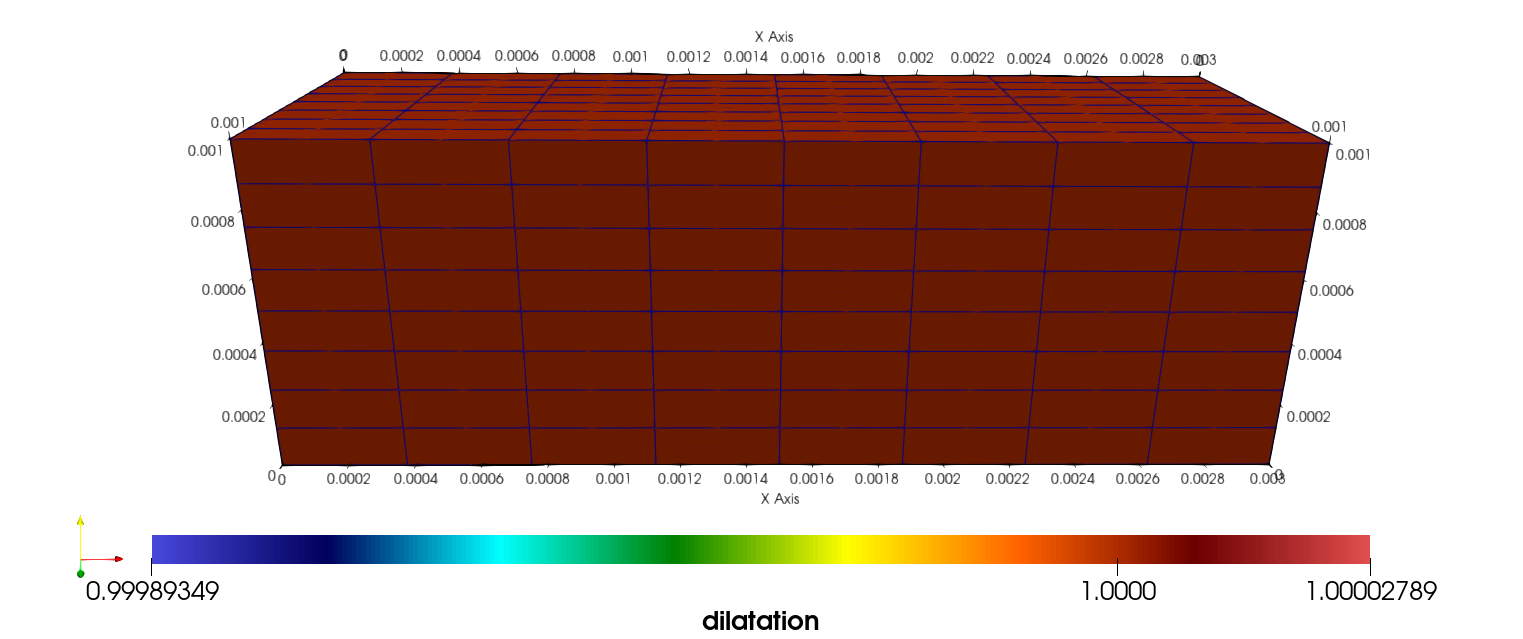
\includegraphics[height=0.18\textheight]{figs/00-D.png}
  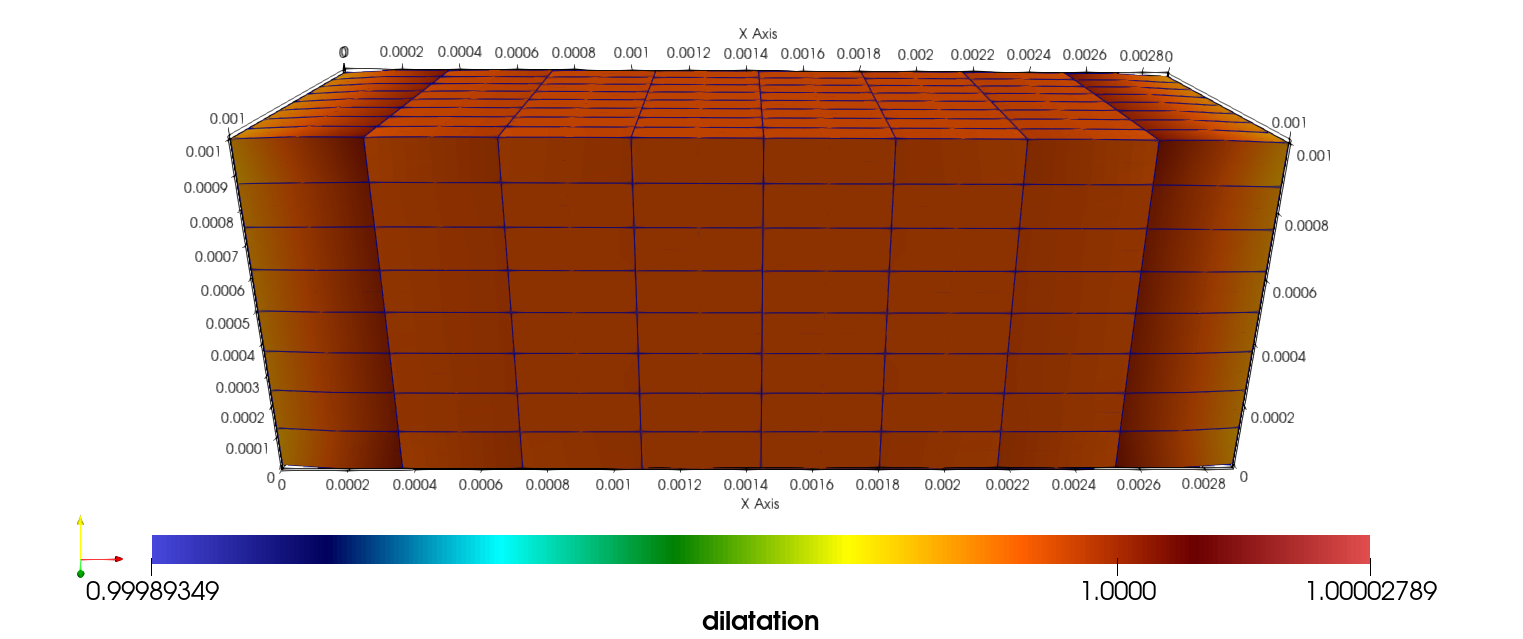
\includegraphics[height=0.18\textheight]{figs/05-D.png}
  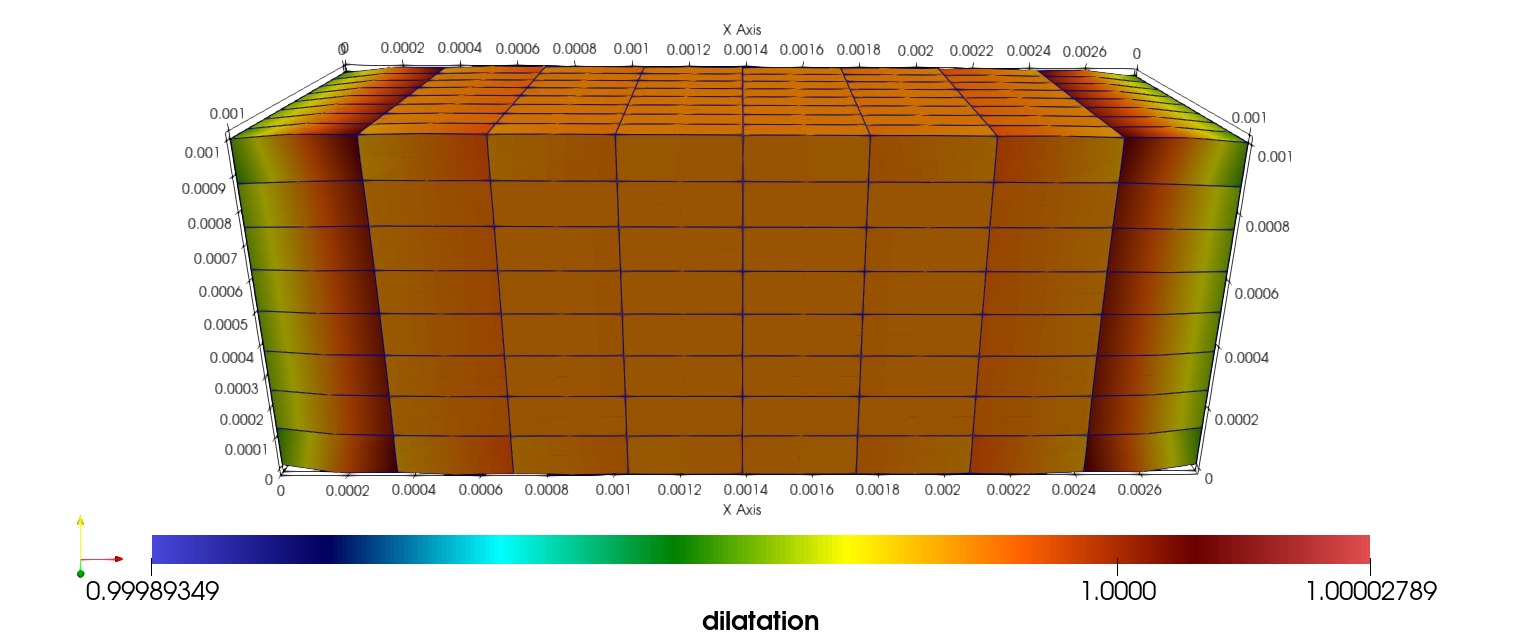
\includegraphics[height=0.18\textheight]{figs/10-D.png}
  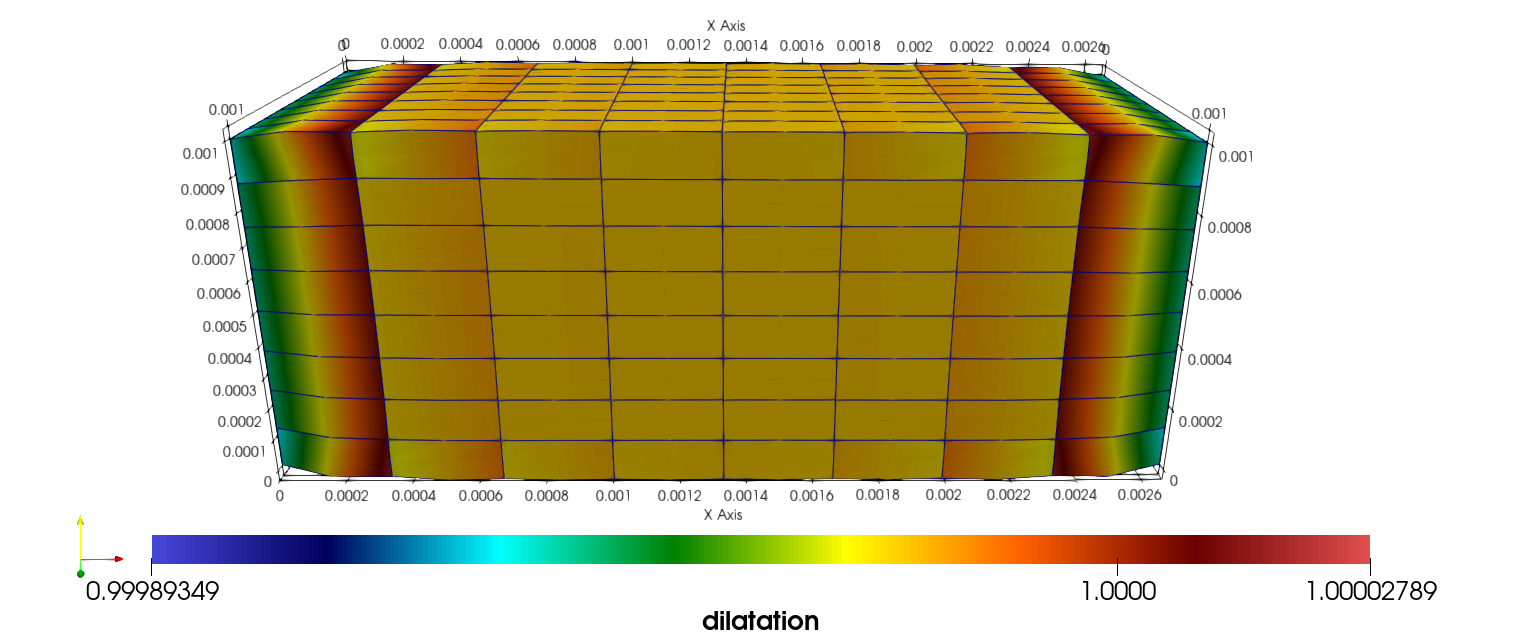
\includegraphics[height=0.18\textheight]{figs/15-D.png}
  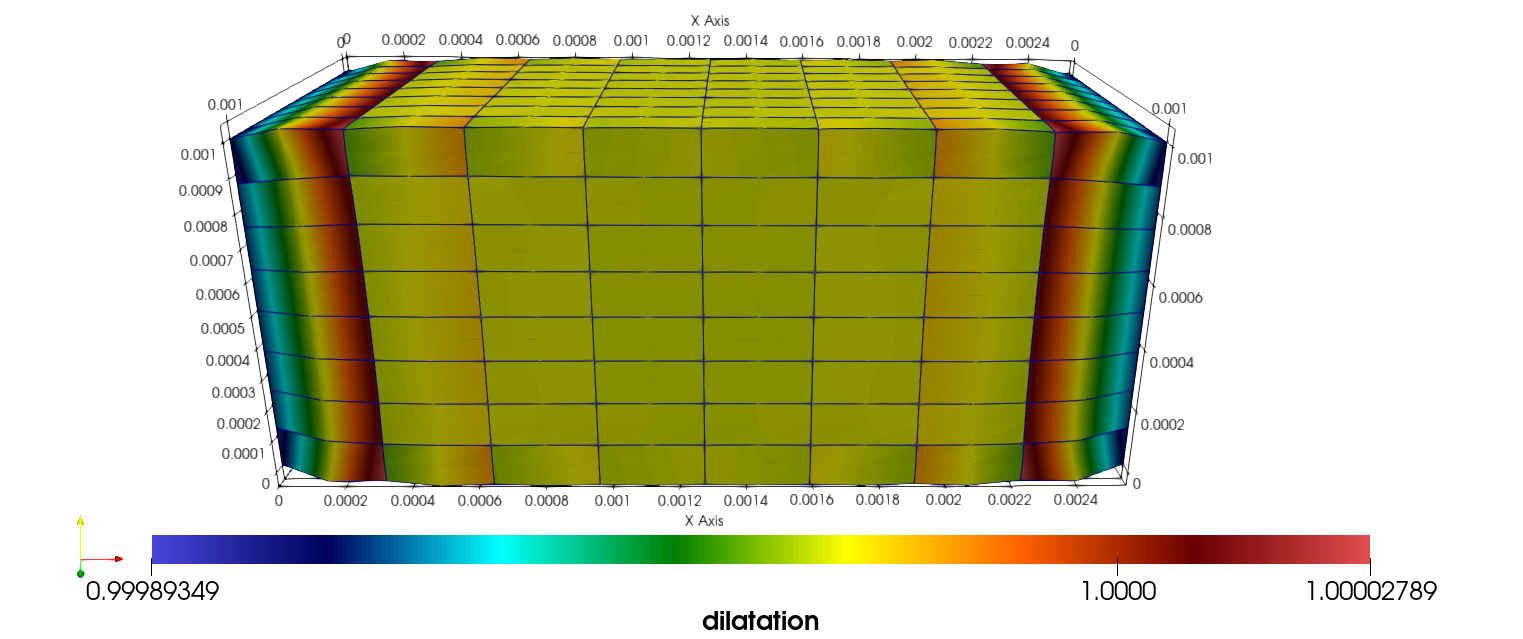
\includegraphics[height=0.18\textheight]{figs/20-D.png}
  \caption{Screenshots of pressure at timesteps 0 of 20, 5 of 20, 10 of 20, 15 of 20, and 20 of 20.}
\end{figure}

\clearpage

\section{Comparative performance of solvers}

The main goal of this section is to document the performance of the different solvers implemented in the code. Recall that, at this juncture, the material is purely Neo-Hookean with no fibre component. This means that the elasticity tensor $\mathbb{C}$ takes a simpler structure given that $\bar{\mathbb{C}}$ is identically zero. This type of experiment could also be thought as passively pulling a block of muscle in which the fibre component has been deactivated.

We repeat the experiment from previous section but set the end time to 0.275. This corresponds to the middle of the linear ramp. Here, report the number of linear iterations, as well as the number of nonlinear iterations. We see from Tables \ref{tab:qs} and \ref{tab:dyn} that only when using CG + ssor the number of nonlinear iterations is 4. All other combinations of solvers complete a time step in 3 nonlinear iterations.

% QUASI-STATIC
\begin{table}
  \centering
  \begin{tabular}{|c|c|c|c|l|} \hline
    SC & Solver & Preconditioner & CPU Time (s) & Linear iterations \\\hline
    False & Direct & - & 62.6 &  1,1,1  \\\hline
    False & CG & ssor & 254.1 & 565, 1039, 1855 \\\hline
    False & CG & jacobi & 78.3 & 1083, 952, 1627 \\\hline
    False & GMRES & ssor & - & Too slow \\\hline
    False & GMRES & jacobi & - & Too slow \\\hline
    True  & Direct & - & 54.8 & 1,1,1 \\\hline
    True  & CG & ssor & 1031.0 & 948, 3748, 5076, 5847 \\\hline
    True  & CG & jacobi & 208.5 & 1875, 3311, 9679 \\\hline
    True  & GMRES & ssor & - & Failed at iteration \#1 \\\hline
    True  & GMRES & jacobi & - & Failed at iteration \#1 \\\hline
  \end{tabular}
  \caption{Comparative performance of implemented solvers for \textit{quasi-static} deformation. \label{tab:qs}}
\end{table}

% Dynamic
\begin{table}
  \centering
  \begin{tabular}{|c|c|c|c|l|} \hline
    SC & Solver & Preconditioner & CPU Time (s) & Linear iterations \\\hline
    False & Direct & - & 144.7 &  1,1,1  \\\hline
    False & CG & ssor & 338.1 & 568, 1022, 1885 \\\hline
    False & CG & jacobi & 163.3 & 1100, 879, 1562 \\\hline
    False & GMRES & ssor & - & Too slow \\\hline
    False & GMRES & jacobi & - & Too slow \\\hline
    True  & Direct & - & 138.3 & 1,1,1 \\\hline
    True  & CG & ssor & 1181.0 & 944, 3757, 5065, 5811 \\\hline
    True  & CG & jacobi & 285.8 & 1875, 3339, 9675 \\\hline
    True  & GMRES & ssor & - & Failed at iteration \#1 \\\hline
    True  & GMRES & jacobi & - & Failed at iteration \#1 \\\hline
  \end{tabular}
  \caption{Comparative performance of implemented solvers for \textit{dynamic} deformation.\label{tab:dyn}}
\end{table}



%%%%%%%%%%%%%%%%%%%%%%%%%%%%%%%%%%%%%%%%%%%%%%%%%%%%%%%%%%%%%
%
%	THE BIBLIOGRAPHY
%
%%%%%%%%%%%%%%%%%%%%%%%%%%%%%%%%%%%%%%%%%%%%%%%%%%%%%%%%%%%%%

\begin{thebibliography}{99} % Use MathSciNet style
\addcontentsline{toc}{chapter}{Bibliography}
\markboth{Bibliography}{Bibliography}

\bibitem{holzapfel}{
{\sc G. A. Holzapfel}. 
{Nonlinear solid mechanics: a continuum approach for engineering science}.
John Wiley \& Sons, Ltd., Chichester, 2000. 
}

\end{thebibliography}




\end{document}
